% Protocolo temporal (Seção Protocolos de avaliação, 03-Metodologia.tex)
% Cores usadas nesta figura (valores CMYK da paleta dvipsnames do xcolor), definidas aqui para não depender de opções externas
\definecolor{RoyalBlue}{cmyk}{1,0.50,0,0}
\definecolor{BurntOrange}{cmyk}{0,0.51,1,0}
\begin{figure}[htbp]
    \centering
    \caption{Protocolo temporal: divisão das \textit{releases} entre treino e teste}
    \label{fig:met-protocolo-temporal}
    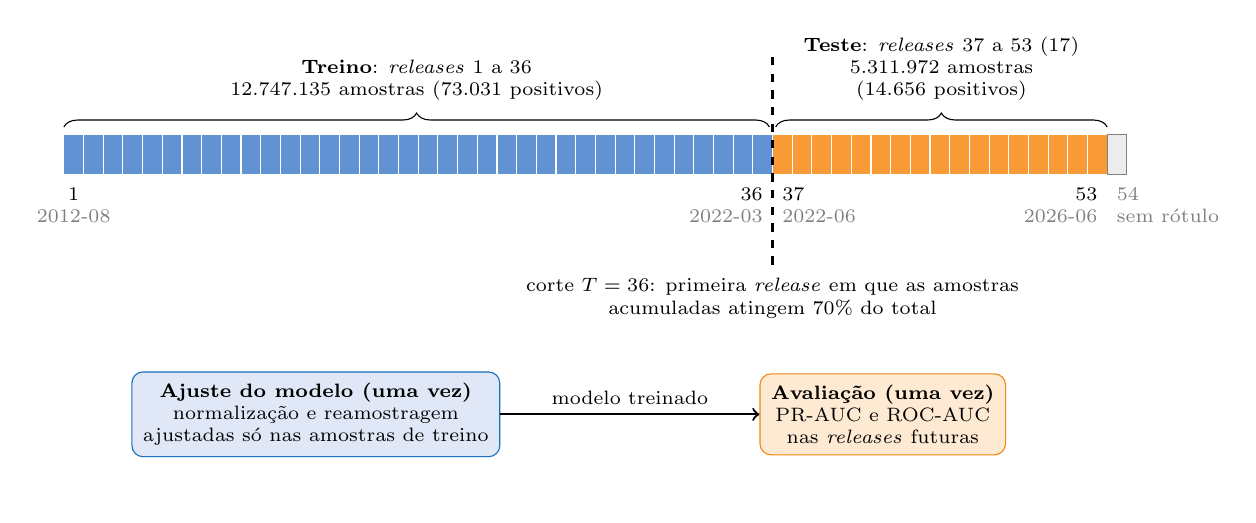
\begin{tikzpicture}[x=1cm,y=1cm,font=\scriptsize,
        caixa/.style={draw,rounded corners,align=center,inner sep=4pt,minimum height=0.9cm},
        chave/.style={decorate,decoration={brace,amplitude=5pt}}]
        \def\w{0.25}
        % ---- releases 1 a 54
        \foreach \i in {1,...,36}{\fill[RoyalBlue!65,draw=white] ({(\i-1)*\w},0) rectangle ++(\w,0.5);}
        \foreach \i in {37,...,53}{\fill[BurntOrange!80,draw=white] ({(\i-1)*\w},0) rectangle ++(\w,0.5);}
        \filldraw[fill=gray!15,draw=gray] ({53*\w},0) rectangle ++(\w,0.5);
        % ---- índices e datas
        \node[anchor=north,align=center] at ({0.5*\w},-0.05) {1\\\textcolor{gray}{2012-08}};
        \node[anchor=north east,align=right] at ({36*\w},-0.05) {36\\\textcolor{gray}{2022-03}};
        \node[anchor=north west,align=left] at ({36*\w},-0.05) {37\\\textcolor{gray}{2022-06}};
        \node[anchor=north east,align=right] at ({53*\w},-0.05) {53\\\textcolor{gray}{2026-06}};
        \node[anchor=north west,align=left,text=gray] at ({53*\w},-0.05) {54\\sem rótulo};
        % ---- corte
        \draw[dashed,thick] (9,-1.15) -- (9,1.53);
        \node[anchor=north,align=center] at (9,-1.2) {corte $T = 36$: primeira \textit{release} em que as {\azul amostras}\\
            acumuladas atingem 70\% do total};
        % ---- chaves
        \draw[chave] (0,0.6) -- ({36*\w-0.04},0.6) node[midway,above=6pt,align=center]
            {\textbf{Treino}: \textit{releases} 1 a 36\\12.747.135 {\azul amostras} (73.031 positivos)};
        \draw[chave] ({36*\w+0.04},0.6) -- ({53*\w},0.6) node[midway,above=6pt,align=center]
            {\textbf{Teste}: \textit{releases} 37 a 53 (17)\\5.311.972 {\azul amostras}\\(14.656 positivos)};
        % ---- fluxo
        \node[caixa,fill=RoyalBlue!12,draw=RoyalBlue] (tr) at (3.2,-3.05)
            {\textbf{Ajuste do modelo (uma vez)}\\normalização e reamostragem\\ajustadas só nas {\azul amostras} de treino};
        \node[caixa,fill=BurntOrange!15,draw=BurntOrange] (te) at (10.4,-3.05)
            {\textbf{Avaliação (uma vez)}\\{\laranja PR-AUC e ROC-AUC}\\nas \textit{releases} futuras};
        \draw[->,thick] (tr) -- node[above]{modelo treinado} (te);
        \node[align=center,text=gray] at (6.8,-3.95)
            {};
    \end{tikzpicture}
    \fonte{Elaborado pelo autor (2026).}
\end{figure}%
